
\documentclass[UKenglish,aspectratio=169]{beamer}

\usepackage{import}
\usepackage{texmex/overhead}



% Options

\newif\ifCompAnims  % Compile animations
\newif\ifOnlyNotes  % Show only notes
\newif\ifShowNotes  % Show notes in the right panel (overrides the others)

% -------

% Set option values
\ShowNotestrue

\CompAnimsfalse

\OnlyNotesfalse


\ifOnlyNotes\ShowNotestrue\CompAnimsfalse\else\fi

% -------


\ifShowNotes
  \setbeameroption{show notes}
  \ifOnlyNotes
    \setbeameroption{show only notes}
  \else
    \setbeameroption{show notes on second screen=right}
  \fi
  \setbeamertemplate{note page}[plain] % removed the thumbnail of the slide
  \setbeamerfont{note page}{size=\fontsize{13}{14}}
  % \setbeamercolor{note page}{bg=uioyellow}
  % \setbeamerfont{beamer-font name}{attributes}
  % \setbeamertemplate{note page}{\pagecolor{yellow!5}\insertnote}
\else\fi



\author{Nanna Bryne}
% \uioemail{dag@ifi.uio.no}
\title{Spacetime Ripples from Domain-Wall Wiggles}
\subtitle{\footnotesize On the analytical prediction of the gravitational-wave signature from perturbed topological defects in expanding spacetime}

\begin{document}

\ifOnlyNotes
\else
\uiofrontpage[dept={Institute of Theoretical Astrophysics},
  info={Master's presentation},
  image={figs/fp_im.png},
  date={12th December 2024},
  smaller]
\fi




% \note{}
{\setbeamercolor{background canvas}{bg=uioblue3}
\begin{frame}[plain,noframenumbering]
  \frametitle{Contents}
  % \(+\)~\textsc{intro}
  \tableofcontents[hideallsubsections]%\note{We will spend most time on the intro. and description of the project.}
  % \(+\)~\textsc{outro}
  % \begin{notes}{0}
  %   \nnote{}{%
  %     1) Aimed at more broad audience, but not expected to explain all concepts.\par
  %     2) Somewhat technical, but should be possible to follow for many. \par
  %     3) Largely a validation analysis, non-physicists will hopefully also keep track\dots \par
  %     4) Closing words, way forward.
  %   }
  % \end{notes}
  % \note[item]{\emph{intro:} Will mostly make sense to those with basic knowledge of the field.}
  % \note[item]{\emph{background:} }
  % \note[item]{\emph{project:} Somewhat technical, but should be possible to follow for many.}
  % \note[item]{\emph{analysis:} Largely a validation analysis, non-physicists will hopefully also keep track\dots}
  % \note[item]{\emph{end:} Closing words, way forward.}
\end{frame}}


% \section*{\textsc{intro}}\label{sec:intro}
% {%\setbeamercolor{background canvas}{bg=uioorange3}
% % \usebackgroundtemplate{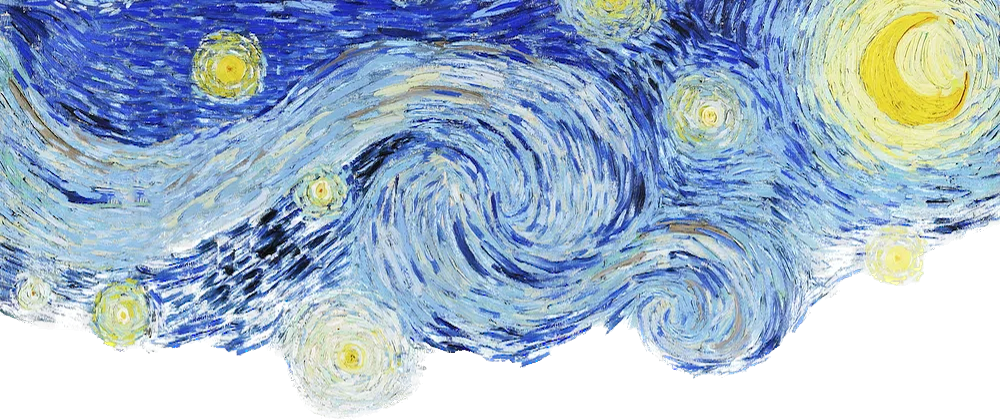
\includegraphics[width=0.5\paperwidth, keepaspectratio]{starry-night.png}}
% \import{sections/}{intro.tex}}


\section{Background}\label{sec:background}
{\import{sections/}{intro.tex}}
{\import{sections/}{background.tex}}



\section{Project}\label{sec:project}
{\import{sections/}{project.tex}}




% SIMULATION COLOURS


\makeatletter

\definecolor{sim@O}{HTML}{214761}        % dark slate blue?
\definecolor{sim@I}{HTML}{3E82FC}        % dodgerblue
\definecolor{sim@II}{HTML}{FE440F}       % orangered
\definecolor{sim@III}{HTML}{9A0EEA}      % violet
\definecolor{sim@IV}{HTML}{020035}       % midnight blue
\definecolor{sim@V}{HTML}{A9F971}        % spring green
\definecolor{sim@VI}{HTML}{E50000}       % red
\definecolor{sim@VII}{HTML}{6E750E}      % olive






% \providecommand*\sim@num[1]{\(\mathnormal{#1}\)}

\providecommand*\sim@num[1]{\(\mathsf{#1}\)}
\providecommand\sim@boxd[2]{\boxed{\sim@num{#1}}}


\providecommand{\simO}{\textcolor{sim@O}{\sim@num{0}}}
\providecommand{\simI}{\textcolor{sim@I}{\sim@num{1}}}
\providecommand{\simII}{\textcolor{sim@II}{\sim@num{2}}}
\providecommand{\simIII}{\textcolor{sim@III}{\sim@num{3}}}
\providecommand{\simIV}{\textcolor{sim@IV}{\sim@num{4}}}
\providecommand{\simV}{\textcolor{sim@V}{\sim@num{5}}}
\providecommand{\simVI}{\textcolor{sim@VI}{\sim@num{6}}}
\providecommand{\simVII}{\textcolor{sim@VII}{\sim@num{7}}}

% \WithSuffix\providecommand{\simO}{\sim@num{0}}



\providecommand{\simnum}{\sim@num}


\makeatother



\section{Analysis}\label{sec:analysis}
{\import{sections/}{analysis.tex}}

\section{Foreground}\label{sec:end}
{\import{sections/}{end.tex}}

% \section*{\textsc{outro}}\label{sec:intro}
% {\setbeamercolor{background canvas}{bg=uioblue3}
% % \usebackgroundtemplate{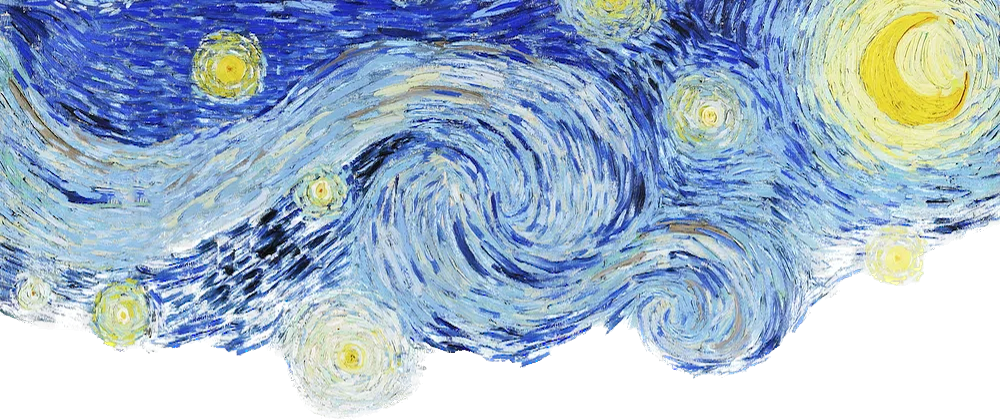
\includegraphics[width=0.5\paperwidth, keepaspectratio]{starry-night.png}}
% \import{sections/}{outro.tex}}



% \section{The end}


% \uiofullpageimage{starry-night.png}
% \uiofullpageimage{starry-night.png}
% \uiofullpageimage{starry-night.png}
% \uiofullpageimage{starry-night.png}


% \begin{frame}{\textcolor{DUMMY1}{DUMMY}}
%   \textcolor{DUMMY1}{%
%   \cite{christiansenGravitationalWavesDark2024,christiansenAsevolutionRelativisticNbody2023,christiansenCosmologicalSimulationsPhase2024,christiansenAsimulationDomainFormation2024}}
%   \textcolor{DUMMY1}{%
%   \cite{hinterbichlerSymmetronCosmology2011,perivolaropoulosGravitationalTransitionsExplicitly2022}}
%   %
% \end{frame}


\section*{Bibliography}
\begin{frame}[plain,noframenumbering]{References}
  \bibliography{../refs}
  \medskip
  \textcolor{uiogrey}{((All figures are created by the author.))}
\end{frame}


\end{document}

